\section{\sys 概览}

\subsection{设计概览}
为了支持集成 DIMM-PIM 的方案，如图~\ref{fig:design-overview} 所示，我们提出由两部分组成的 \sys：
(1) \sys-PIM，即我们为高效执行 Attention 专门设计的 DIMM-PIM 硬件；以及
(2) \sys-sys，即一个可扩展的 AFD 系统，它协调 GPU 与 \sys-PIM 上的计算，目标是最大化推理吞吐量。

\myparagraph{\sys 的推理工作流。}
\sys-sys 沿用子批次调度技术~\cite{heo2024neupims,jiang2024neo}，在每轮迭代中选择请求组成子批次。
起初，每个子批次中所有请求的 QKV 生成会被批处理并在 GPU 上执行。
随后，预填充 Attention 与解码 Attention 分别在 GPU 和 \sys-PIM 上并发处理。
\sys 汇聚批次内所有请求的 Attention 输出，再批量执行后续操作（投影、前馈等）。
GPU 与 \sys-PIM 通过 PCIe 互连。

\myparagraph{解决 DIMM-PIM 集成挑战。}
如第~\ref{sec:intro} 节所述，集成 DIMM-PIM 会带来架构分离以及随之而来的同步开销：
在 DIMM 内部，分布式芯片会同时产生数据同步与布局同步代价；DIMM-PIM 与 GPU 的分离则增加跨设备数据同步和进度同步开销。
为解决前一类问题，\sys-PIM 采用无气泡流水线（第~\ref{sec:design-dp-pipeline} 节）和混合粒度重布局（第~\ref{sec:design-dp-relayout} 节）；
为解决后一类问题，\sys-sys 采用秩组粒度通信--计算重叠（第~\ref{sec:design-sys-comm} 节）和对齐预测调度（第~\ref{sec:sys-scheduler} 节）。

\begin{figure}[t]
  \setlength{\abovecaptionskip}{1.2pt}
  \setlength{\belowcaptionskip}{-15pt}
  \centering
  \begin{minipage}[t]{0.92\linewidth}
    \centering
    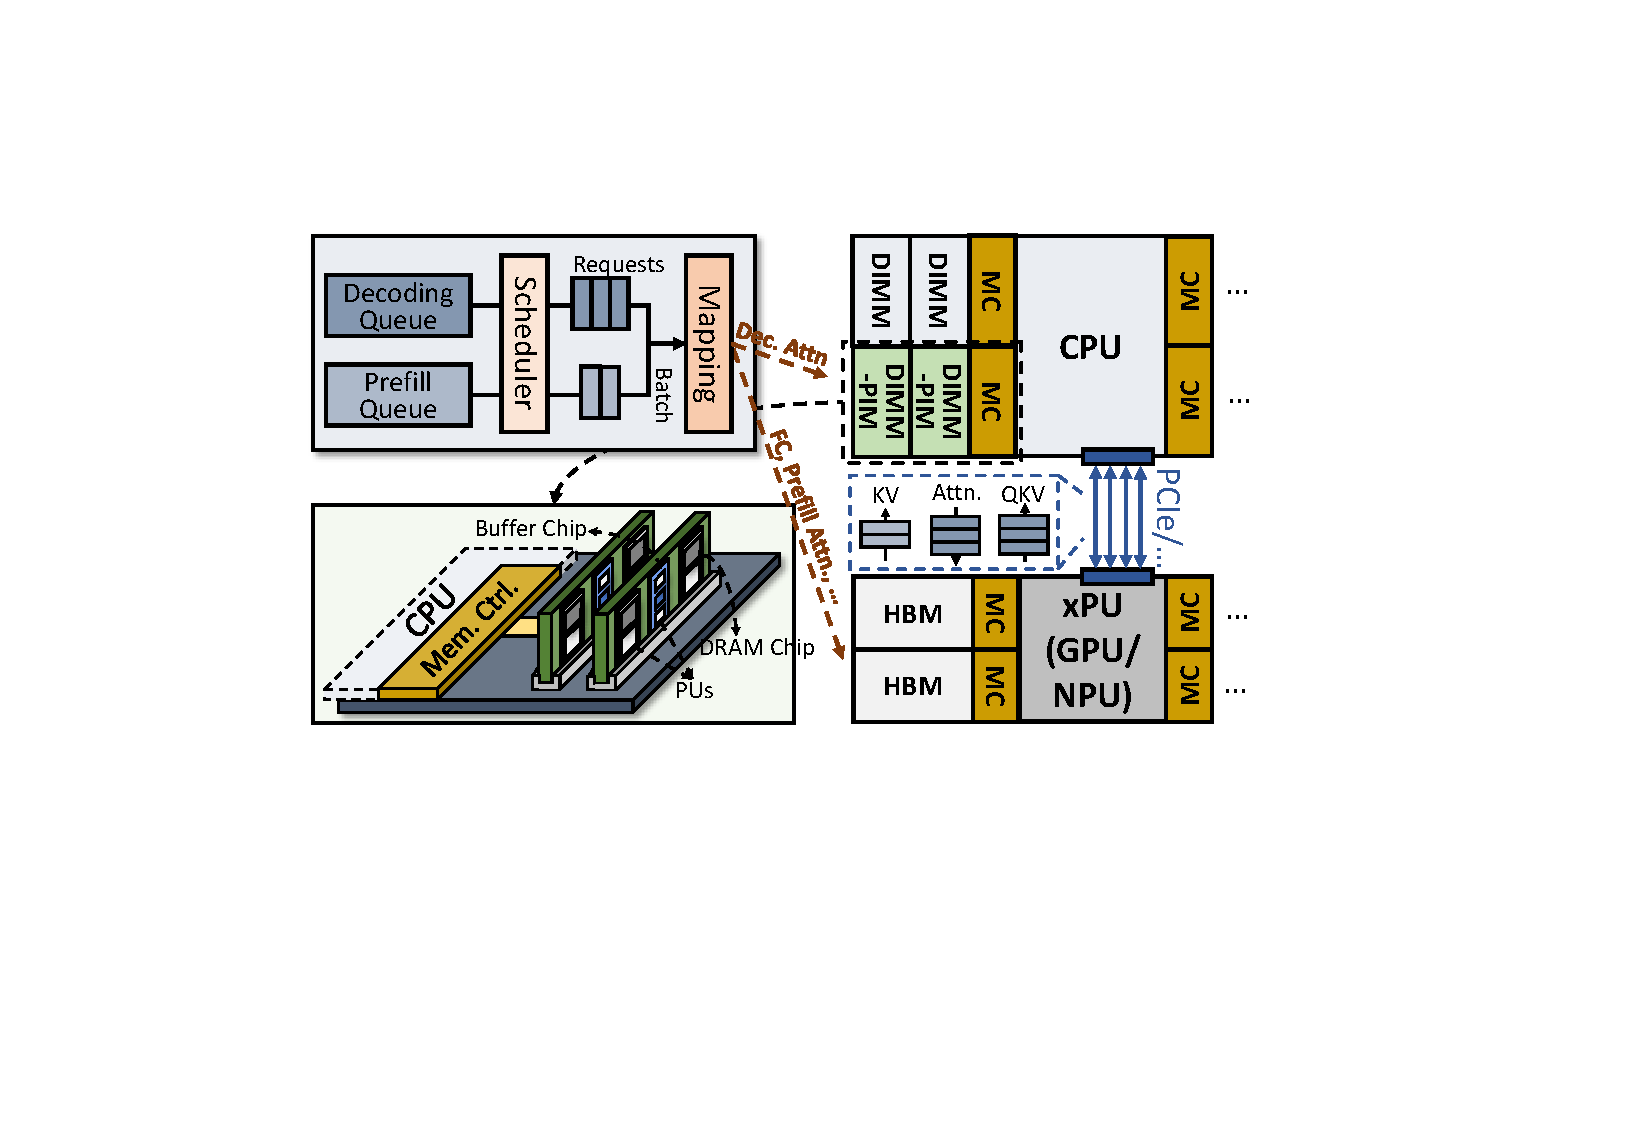
\includegraphics[width=\textwidth]{figs/design-overview.pdf}
    \footnotesize
  \end{minipage}
  \caption{\textbf{\sys 概览。}}
  \label{fig:design-overview}
\end{figure}
